% Se configura el tipo de documento
\documentclass[a4paper]{scrartcl}

%THIS IS TO MAKE THE DOCUMENT PRETTIER
\usepackage[utf8]{inputenc}
\usepackage[spanish, es-tabla, es-nodecimaldot]{babel}

\usepackage[T1]{fontenc}
\usepackage{lmodern} %AGREGO1
\usepackage{fourier}			% English language/hyphenation

\usepackage{color}
\usepackage[protrusion=true,expansion=true]{microtype}
\usepackage{amsmath}
\usepackage{amsfonts,amsthm} % Math packages
\usepackage[pdftex]{graphicx}
\usepackage{url}
\usepackage{import}
\usepackage{multicol}

\usepackage[margin=2cm]{geometry}

% %%% Custom sectioning
\usepackage{sectsty}
\allsectionsfont{\normalfont \scshape} 

%%% Custom headers/footers (fancyhdr package)
\usepackage{fancyhdr}
\pagestyle{fancyplain}

\fancyhead{}											% No page header
\fancyfoot[L]{}											% Empty
\fancyfoot[C]{}											% Empty
\fancyfoot[R]{\thepage}									% Pagenumbering
\renewcommand{\headrulewidth}{0pt}			% Remove header underlines
\renewcommand{\footrulewidth}{0pt}				% Remove footer underlines
\setlength{\headheight}{13.6pt}

\usepackage{float}

%%% Equation and float numbering
\numberwithin{equation}{section}		% Equationnumbering: section.eq#
\numberwithin{figure}{section}			% Figurenumbering: section.fig#
\numberwithin{table}{section}				% Tablenumbering: section.tab#

%%% Maketitle metadata
\newcommand{\horrule}[1]{\rule{\linewidth}{#1}} 	% Horizontal rule
%FINISHED MAKING PRETTIER DOCUMENT



% --------------ADDED BY FACUNDO FARALL--------------

%MATHEMATICS PACKAGES
\usepackage{amsmath,amsfonts,amsthm}
%FINISHED MATHEMATICS



%THIS IS SO THAT REFERENCES CAN BE CLICKED
\usepackage{hyperref}
\hypersetup{
    colorlinks=true,
    linkcolor=blue,
    filecolor=magenta,      
    urlcolor=blue,
    citecolor=blue,    
}
%FINISHED CLICKABLE REFERENCES



%THIS IS TO CHANGE MARGINES FOR SITUATIONS LIKE LONG EQUATIONS
\usepackage[strict]{changepage}
%ENDS CHANGER OF MARGINS



%THIS IS TO USE SMALLER FONT SIZE
\usepackage[11pt]{moresize}
%FINISHED FONT SIZE CHANGER



%THE FOLLOWING ARE CONFIGURATIONS FOR TODONOTES
\usepackage{todonotes,varwidth}
\makeatletter
\tikzstyle{diaanotestyle} = [
    draw=\@todonotes@currentbordercolor,
    fill=\@todonotes@currentbackgroundcolor,
    line width=0.5pt,
    inner sep = 0.8 ex,
    rounded corners=4pt,align=left,
   ]

\renewcommand{\@todonotes@drawInlineNote}{%
        {\begin{tikzpicture}[remember picture,baseline={(0,0)}]%
            \draw node[diaanotestyle,font=\@todonotes@sizecommand,anchor=base west]{%
               \begin{varwidth}[t]{10cm}
                \if@todonotes@authorgiven%
                    {\@todonotes@sizecommand \@todonotes@author:\,\@todonotes@text}%
                \else%
                    {\@todonotes@sizecommand \@todonotes@text}%
                \fi
                \end{varwidth}};%
            \end{tikzpicture}}%
       }%
\makeatother
%HERE ENDS THE CONFIGURATIONS FOR TODONOTES

% --------------ENDS ADDED BY FACUNDO FARALL--------------

\begin{document}

\title{
	\usefont{OT1}{bch}{b}{n}
	\normalfont \normalsize \textsc{Instituto Tecnol\'ogico de Buenos Aires} \\ [25pt]
	\horrule{2pt} \\[0.4cm]
	\huge Trabajo Pr\'actico Nº 1\\ Configuraci\'on Darlington \\
	\horrule{2pt} \\[0cm]
\author{\\Grupo 2:\\\\Francois, Mat\'ias\\Maselli, Carlos\\ M\"uller, Malena\\ Trozzo, Nicol\'as\\ \\ \\ \\
Profesores: \\\\ Alcocer, Fernando\\ Oreglia, Eduardo Victor \\Gardella, Pablo Jes\'us\\ \\ } 
\text{Electr\'onica I - 2019}
}
\date{\today} 
\pagenumbering{arabic}

\maketitle
\newpage

\section{Introducci\'on}

La configuraci\'on ''Darlington'', tambi\'en conocida como ''par Darlington'', consiste en dos transistores conectados como se observa en la figura \ref{darlington_ideal}, con el fin de obtener una mayor ganancia de corriente respecto a la obtenida al emplear un \'unico transistor. En este trabajo se analiza el comportamiento del circuito \ref{darlington_tp} para comprender la utilidad del par Darlington.

\begin{figure}[H]
	\centering
		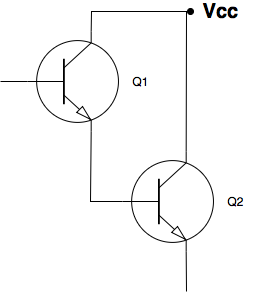
\includegraphics[scale=0.4]{../darlington_ideal.png} 
	\caption{Configuraci\'on Darlington.}
	\label{darlington_ideal}
\end{figure}

\begin{figure}[H]
	\centering
		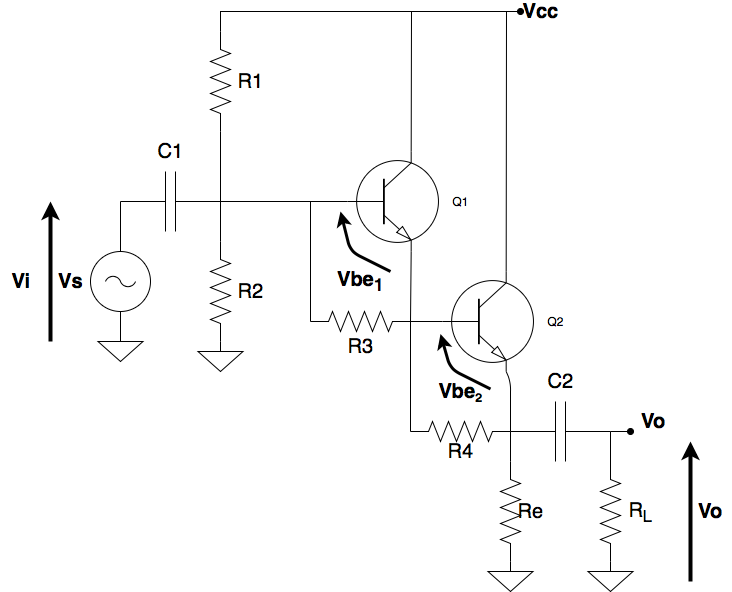
\includegraphics[scale=0.4]{../darlington_tp.png} \\
	\caption{Circuito de estudio en este trabajo, implementando un par Darlington.}
	\label{darlington_tp}
\end{figure}

%\begin{figure}[H]
%	\centering
%	\begin{tabular}{c c}
%		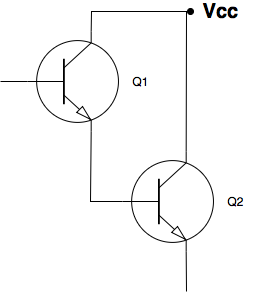
\includegraphics[scale=0.3]{../darlington_ideal.png} &
%		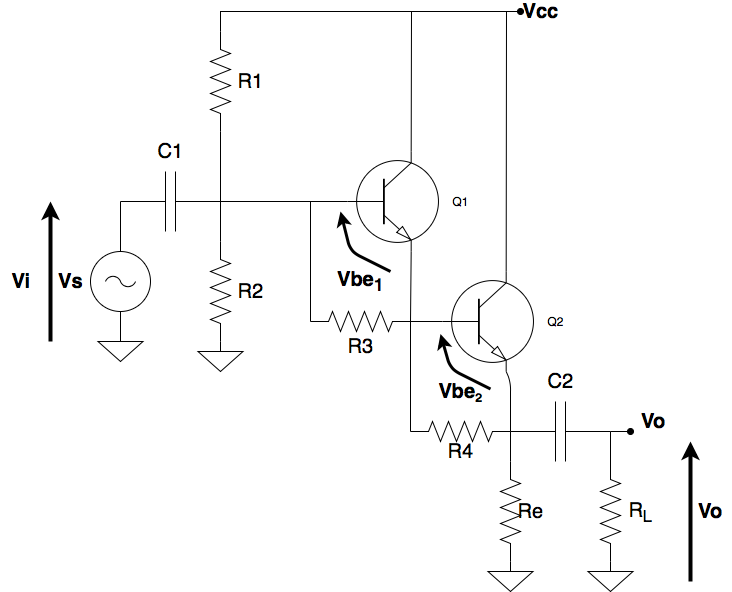
\includegraphics[scale=0.3]{../darlington_tp.png} \\
%	\end{tabular}
%	\caption{}
%	\label{darlington_tp}
%\end{figure}

\section{An\'alisis te\'orico del circuito}

	\subsection{Polarizaci\'on}
		
		\begin{figure}[H]
			\centering
			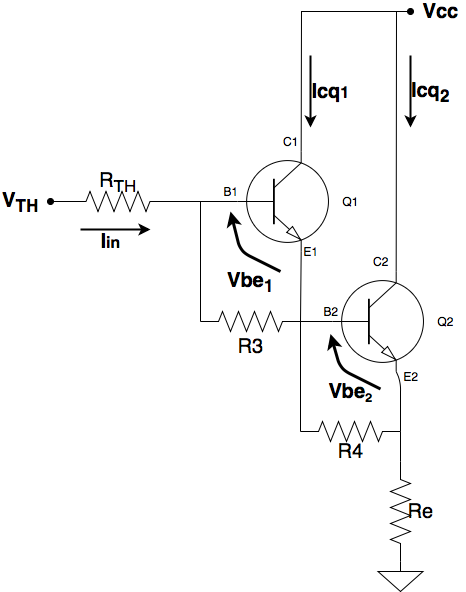
\includegraphics[scale=0.4]{../polarizacion.png} \\
			\caption{Circuito equivalente para el an\'alisis de polarizaci\'on.}
			\label{polarizacion}
		\end{figure}

	\begin{equation}	
		\begin{cases}
		V_{TH} = \frac{R_2}{R_1 + R_2} V_{CC}\\ \\
		R_{TH} = R_1 // R_2
		\end{cases}
		\label{Thevenin}
	\end{equation}
	
	\begin{equation}
	\begin{cases}
		V_{TH} -  R_{TH} I_{TH} - Vbe_1 - Vbe_2 -(Ie_2 + I_{R4})Re = 0\\ \\
		I_{TH} = Ib_1 + \frac{Vbe_1}{R_3}\\ \\
		Ie_2 = (HFE_2 + 1)Ib_2\\ \\
		Ib_2 = \frac{Vbe_1}{R_3} + (HFE_1+1)Ib_1 - \frac{Vbe_2}{R_4}
		\end{cases}
	\end{equation}
	
		\begin{equation}
	\begin{cases}
	Ic_1 = (HFE_1 + 1)Ib_1\\ \\
	Ic_2 = HFE_2 (\frac{Vbe_1}{R_3} + (HFE_1 + 1)Ib_1 - \frac{Vbe_2}{R_4})
	\end{cases}
	\end{equation}
	
	\todo{Seguir pasando en limpio las ecs de polarizacion y explicar paso a paso}

	\subsection{Modelo incremental}
	
		\begin{equation}
			\begin{cases}
			\widehat{r}_{aux} = \frac{V_T}{I_{cq}}\\
			\widehat{g}_m = \frac{1}{r_{aux}}\\	
			\widehat{h}_{ie} = (h_{fe} + 1) r_{aux}\\
			\widehat{r}_{ce} = \frac{1}{h_{oe}} = \frac{V_A}{I_{cq}}
			\end{cases}
			\label{mod_inc_ecs}
		\end{equation}
	
	Particularmente, para el transistor $Q1$ se emplean las ecuaciones \ref{mod_inc_ecs} con $I_{cq1}$ y $h_{fe1}$, mientras que para el transistor $Q2$ con $I_{cq2}$ y $h_{fe2}$. Se obtienen los siguientes valores:
	
	\todo{COMPLETAR TABLA de estimadores}
	\begin{table}[h!]
		\centering
		\begin{tabular}{c c c}%
			\bfseries Estimadores & Q1 & Q2 \\ \hline
			$\widehat{g}_m$ &  & \\
			$\widehat{h}_{ie}$ &  & \\
			$\widehat{r}_{ce}$&  & \\
			\hline
		\end{tabular}
		\caption{Estimadores correspondientes al modelo incremental, para los transistores Q1 y Q2.}
		\label{avolf}
	\end{table}
	
	\subsection{Circuito incremental}
	
		\begin{figure}[H]
			\centering
			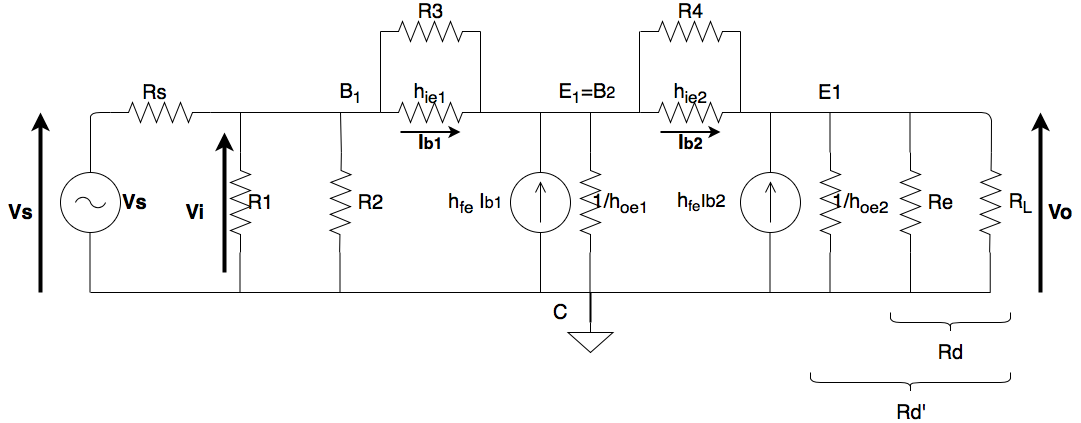
\includegraphics[scale=0.4]{../circ_incremental.png} \\
			\caption{Circuito equivalente para el an\'alisis del circuito incremental.}
			\label{circ_incremental}
		\end{figure}

\section{Diseño del circuito}

\section{Mediciones y resultados obtenidos}

\section{Conclusi\'on}



\end{document}